\section{Modelagem da Troca de Eventos e da Comunicação Entre \glspl{vm} e \glspl{vmm}}

\subsection{Modelagem Formal da Transformação de Eventos Entre Domínios Distintos}

A transformação de um evento do domínio do hospedeiro para o domínio dos convidados, e vice-versa, pode ser formalmente modelada como uma composição de funções parciais.

Considere os conjuntos que representam o universo de eventos processáveis em cada domínio:
\begin{equation}
E_{\mathrm{Hypervisor}} = \{\, e \mid e \text{ é um evento gerado ou tratável pelo sistema hospedeiro} \,\}
\end{equation}
\begin{equation}
E_{\mathrm{Virtual}} = \{\, v \mid v \text{ é um evento gerado ou tratável pelo sistema convidado} \,\}
\end{equation}

Define-se, então, a função que maperia um evento $h \in E_{\mathrm{Hypervisor}}$ para um evento $v \in E_{\mathrm{Virtual}}$ como:

\begin{equation}
\mathcal{F} : E_{\mathrm{Hypervisor}} \rightarrow E_{\mathrm{Virtual}}
\end{equation}

tal que:

\begin{equation}
\mathcal{F}(h) = \mathrm{Inject}(\mathrm{Translate}(\mathrm{Intercept}(h))), \quad \forall h \in E_{\mathrm{Hypervisor}}
\end{equation}

onde:

\begin{itemize}
    \item $\mathrm{Intercept}(\cdot)$: representa a captura do evento pelo hipervisor;
    \item $\mathrm{Translate}(\cdot)$: corresponde à adaptação semântica e estrutural do evento.
    \item $\mathrm{Inject}(\cdot)$: indica a inserção controlada do evento nos ambientes virtualizados.
\end{itemize}

Por outro lado,  a função que mapeia um evento $v \in E_{\mathrm{Virtual}}$ para um evento $h \in E_{\mathrm{Hypervisor}}$ pode ser definida como:

\begin{equation}
\mathcal{G} : E_{\mathrm{Virtual}} \rightarrow E_{\mathrm{Hypervisor}}
\end{equation}

tal que:

\begin{equation}
\mathcal{G}(v) = \mathrm{Dispatch}(\mathrm{Translate}(\mathrm{Intercept}(v))), \quad \forall v \in E_{\mathrm{Virtual}}
\end{equation}

onde:

\begin{itemize}
\item $\mathrm{Dispatch}(\cdot)$: representa a submissão operacional de um evento ao hardware hospedeiro.
\end{itemize}

\subsection{Direcionamento e Virtualização de Interrupções Temporais}

No domínio do hipervisor, eventos temporais resumem-se a interrupções temporais oriundas do hardware de temporização da plataforma. Essas interrupções podem ser transformadas
para os convidados através de uma especialização da função de transformação definida anteriormente. Nesse contexto, as interrupções do temporizador --- originadas no hardware ---
são interceptadas pelo hipervisor, processadas pelo subsistema de temporização e posteriormente injetadas no contexto das CPUs virtuais.

O fluxo de transformação dessas interrupções pode ser modelado como uma especialização da função $\mathcal{F}$, restringindo o seu domínio para o subconjunto das interrupções temporais
$E_{\mathrm{TemporalHypervisor}} \subset E_{\mathrm{Hypervisor}}$. Para uma interrupção de temporizador $e_t \in E_{\mathrm{TemporalHypervisor}}$, a função de transformação é refinada
como $\mathcal{F_T}$, na qual sua definição é dada por:

\begin{equation}
\mathcal{F_T} : E_{\mathrm{TemporalHypervisor}} \rightarrow E_{\mathrm{TemporalVirtual}}
\end{equation}

onde:

\begin{equation}
\mathcal{F_T}(e_t) = \mathrm{Inject_{T}}(\mathrm{Translate_{T}}(\mathrm{Intercept_{T}}(e_{t}))), \quad \forall e_t \in E_{\mathrm{TemporalHypervisor}}
\end{equation}

tal que:

\begin{itemize}
    \item $\mathrm{Intercept}_T(\cdot)$: representa a captura da interrupção pelo hipervisor;
	\item $\mathrm{Translate}_T(\cdot)$: consiste na etapa em que o subsistema responsável pode aplicar alterações no evento, como fatores de escala temporal,
	viabilizando a execução da \gls{vm} sob uma abstração de tempo independente do tempo físico da máquina hospedeira;
    \item $\mathrm{Inject}_T(\cdot)$: representa a etapa final na qual o evento é entregue à \gls{vm} através da geração de uma interrupção virtual.
\end{itemize}

Na prática, esse processo ocorre em múltiplas etapas. A interrupção é inicialmente gerada pelo hardware físico
e interceptada pelo \textit{Trap Handler}. Em seguida, o \textit{Timer} processa a interrupção e a encaminha para a \textit{Virtual CPU}. Por fim, a interrupção é convertida em uma
interrupção virtual e injetada no sistema convidado. O fluxo completo desse mecanismo é ilustrado na Figura~\ref{fig:timer-irq-flow}.

\vspace{0.4cm}

 \begin{center}
    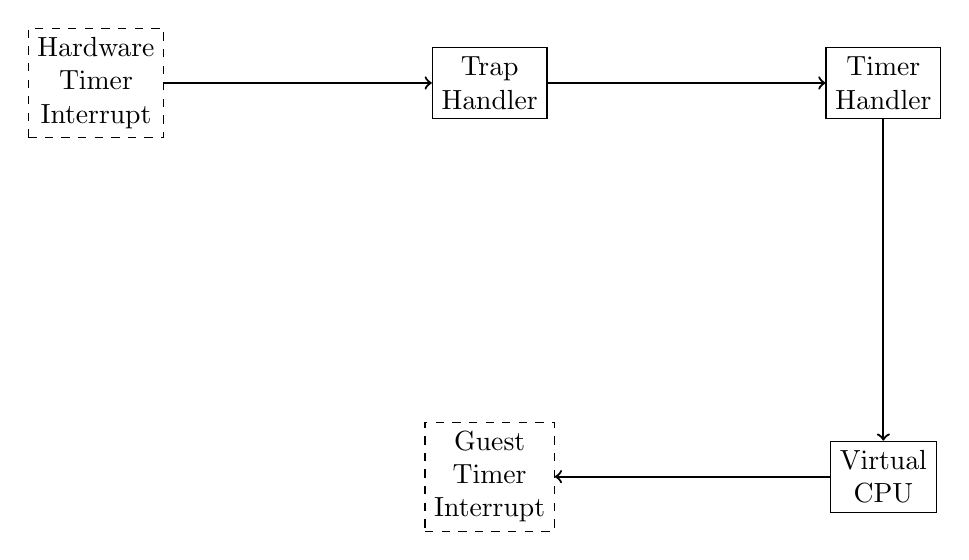
\begin{tikzpicture}
        \node[draw, rectangle, align=center, dashed] (A) at (0,5){Hardware\\Timer\\Interrupt};
        \node[draw, rectangle, align=center] (B) at (5,5){Trap\\Handler};
        \node[draw, rectangle, align=center] (C) at (10,5){Timer\\Handler};
        \node[draw, rectangle, align=center] (D) at (10,0){Virtual\\CPU};
        \node[draw, rectangle, align=center, dashed] (E) at (5,0){Guest\\Timer\\Interrupt};
		\draw[->, thick] (A) -- (B);
        \draw[->, thick] (B) -- (C);
        \draw[->, thick] (C) -- (D);
        \draw[->, thick] (D) -- (E);
		\label{fig:timer-irq-flow}
    \end{tikzpicture}
\end{center}



%\begin{align}
%\mathrm{Intercept}_{T} &: E_{\mathrm{Temporal}} \rightarrow E_{\mathrm{Hypervisor}}, \\
%\mathrm{Translate}_{T} &: E_{\mathrm{Hypervisor}} \rightarrow E_{\mathrm{Virtual}}, \\
%\mathrm{Inject}_{T} &: E_{\mathrm{Virtual}} \rightarrow E_{\mathrm{VM}}.
%\end{align}
%
%com execução sequencial dada por:
%\[
%\mathcal{F}(e_t) = \mathrm{Inject}_{T}(\mathrm{Translate}_{T}(\mathrm{Intercept}_{T}(e_t))).
%\]

%Seja $e_{\mathrm{t}} \in E_{\mathrm{Temporal}}$ um evento temporal detectável pelo hipervisor, o caminho desse evento até ser detectável pelo convidado é dado pela seguinte equação:

%\begin{equation}
%e_{\mathrm{trap}} = \mathrm{TrapHandler}(\mathrm{vCPU}(\mathrm{Intercept}(e_{\mathrm{irq}})))
%\end{equation}


%
%
%\begin{equation}
%E_{hw} \rightarrow E_{trap} \rightarrow E_{vmm} \rightarrow E_{guest}
%\end{equation}
%
%onde:
%\begin{itemize}
%    \item $E_{hw}$ representa eventos originados no hardware;
%    \item $E_{trap}$ representa eventos interceptados pela camada de exceção;
%    \item $E_{vmm}$ representa eventos processados pela camada de virtualização;
%    \item $E_{guest}$ representa eventos entregues ao sistema convidado.
%\end{itemize}
%
%A camada de virtualização atua como uma função de mapeamento:
%\begin{equation}
%Inject(vCPU, event_{host}) \rightarrow event_{guest}
%\end{equation}



%\subsection{Direcionamento e Tratamento de Interrupções Provenientes de Dispositivos Externos}
%
%\begin{center}
%	\begin{tikzpicture}
%		\node[circle, draw, minimum size=2.2cm, align=center, dashed] (A) at (4,0){External\\Device\\Interrupt};
%		\node[circle, draw, minimum size=2.2cm, align=center] (B) at (4,4){Trap\\Handler};
%		\node[circle, draw, minimum size=2.2cm, align=center] (C) at (8,4){Device\\Driver};
%		\node[circle, draw, minimum size=2.2cm, align=center] (D) at (12,4){VirtIO\\Device\\Driver};
%		\node[circle, draw, minimum size=2.2cm, align=center] (E) at (16,4){Virtual\\Machine};
%		\node[circle, draw, minimum size=2.2cm, align=center] (F) at (16, 0){Virtual\\CPU};
%		\node[circle, draw, minimum size=2.2cm, align=center, dashed] (G) at (12,0){Guest\\External\\Device\\Interrupt};
%		\draw[->, thick] (A) -- (B);
%		\draw[->, thick] (B) -- (C);
%		\draw[->, thick] (C) -- (D);
%		\draw[->, thick] (D) -- (E);
%		\draw[->, thick] (E) -- (F);
%		\draw[->, thick] (F) -- (G);
%	\end{tikzpicture}
%\end{center}
%
%\subsection{Processamento de Notificações de \gls{mmio} originadas no \gls{so} Convidado}
%
%\begin{center}
%\begin{tikzpicture}
%\node[circle, draw, minimum size=2.2cm, align=center, dashed] (A) at (4,0){VirtIO\\\gls{mmio}\\Notification};
%\node[circle, draw, minimum size=2.2cm, align=center] (B) at (4,4){Trap\\Handler};
%\node[circle, draw, minimum size=2.2cm, align=center] (C) at (8,4){Virtual\\CPU};
%\node[circle, draw, minimum size=2.2cm, align=center] (D) at (12,4){Virtual\\Machine};
%\node[circle, draw, minimum size=2.2cm, align=center] (E) at (16,4){VirtIO\\Device\\Driver};
%\node[circle, draw, minimum size=2.2cm, align=center] (F) at (16,0){Device\\Driver};
%\draw[->, thick] (A) -- (B);
%\draw[->, thick] (B) -- (C);
%\draw[->, thick] (C) -- (D);
%\draw[->, thick] (D) -- (E);
%\draw[->, thick] (E) -- (F);
%\end{tikzpicture}
%\end{center}


